%=========================================================================

\chapter{Introduction}

When does a machine \textquotedblleft understand\textquotedblright\ an image? One definition could be the following sentence: \emph{A machine understand an image, when in can describe important content of the image.} This description should include present objects, their attributes and relation to each other. Determining the important content of the image can be quite difficult, even for humans, which have been trained for this task since they were born. However, deep learning techniques are proving to be quite successful in this kind of tasks. Similarly to people, these models require large amounts of training data, but later they can evaluate correctly even yet unseen situations.

Deep machine learning, sometimes under the name of neural networks\footnote{Terms \emph{deep learning} and \emph{neural networks} will be used in this work interchangeably.}, is branch of machine learning based on composing multiple non-linear functions to solve the task. As it is fundamentally different from the standard computer algorithms, it perform well on problems, which are unsuitable these algorithms. For example, neural networks have excellent performance in recognizing speech and images, writing stories and composing music. This work focuses on generating image descriptions in regular English sentences, which is also a task suitable for deep learning.

First, in chapter \ref{chp:nn}, I will first introduce neural networks and several key concepts which are used later in this work. In chapter \ref{chp:captions} current state-of-the-art in the field of image captioning and summary of the key papers will be presented. I will list most popular frameworks and libraries for implementation of deep learning models and mention my experiments with them in the chapter \ref{chp:exper}. Using knowledge of previous chapters I will propose an image captioning model in chapter \ref{chp:model}. Expectations of this proposal will be discussed in the concluding chapter \ref{chp:conclusion}.

\chapter{Neural networks} \label{chp:nn}
General idea of artificial neural networks emerged after World War II. Perceptron, as a single neuron unit, was created in 1958 by Frank Rosenblatt\cite{rosenblatt58a}, but became popular only after combination with the backpropagation algorithm\cite{bryson1975applied,werbos1974beyond}. At that time neural nets have not reached massive popularity, not because they are not working, but due to small computing power of machines back then and lack of datasets. Recently (after 2000) neural nets became popular again, under the name of \textquotedblleft deep learning\textquotedblright, to emphasize the use of several layers stacked on top of each other to create deep architectures, which are far more practical than shallow ones. During this reinvention, neural nets have been successfully applied in multiple fields like computer vision\cite{DBLP:journals/corr/HeZRS15}, speech recognition\cite{DBLP:journals/corr/abs-1303-5778} and natural language modeling\cite{DBLP:conf/interspeech/MikolovKBCK10}.

Various useful architectures and algorithms are now introduced almost every month. In this chapter, I will describe only a handful -- recurrent neural networks with the LSTM and GRU units, and basics of convolutional neural nets.

	\section{Recurrent neural nets}
Feedforward neural nets are extremely powerful models, which can be highly parallelized. Despite that, they can be only applied to problems with inputs and outputs, which have fixed dimensionality (e.g. one-hot encoding vectors). This is a serious drawback, as many of the real-world problems are defined as sequences with lengths that are unknown to us in beforehand. Soon recurrent neural networks were introduced and they proved to be very useful to this kind of task. There is vast amount of recurrent neural networks, many not suitable for sequential tasks like Hopfield network, which are very successful in specific tasks, but nevertheless not useful for us now.

Apart from classification, which can be more precise when using sequences, one of the most important tasks is next value prediction. This core task can be then extended very simply to predict arbitrary number of future values. Prediction problems are all around us, from the weather forecast and stock market prediction to the autocomplete in smartphones or web browsers.

\begin{figure}[!ht]
	\centering
	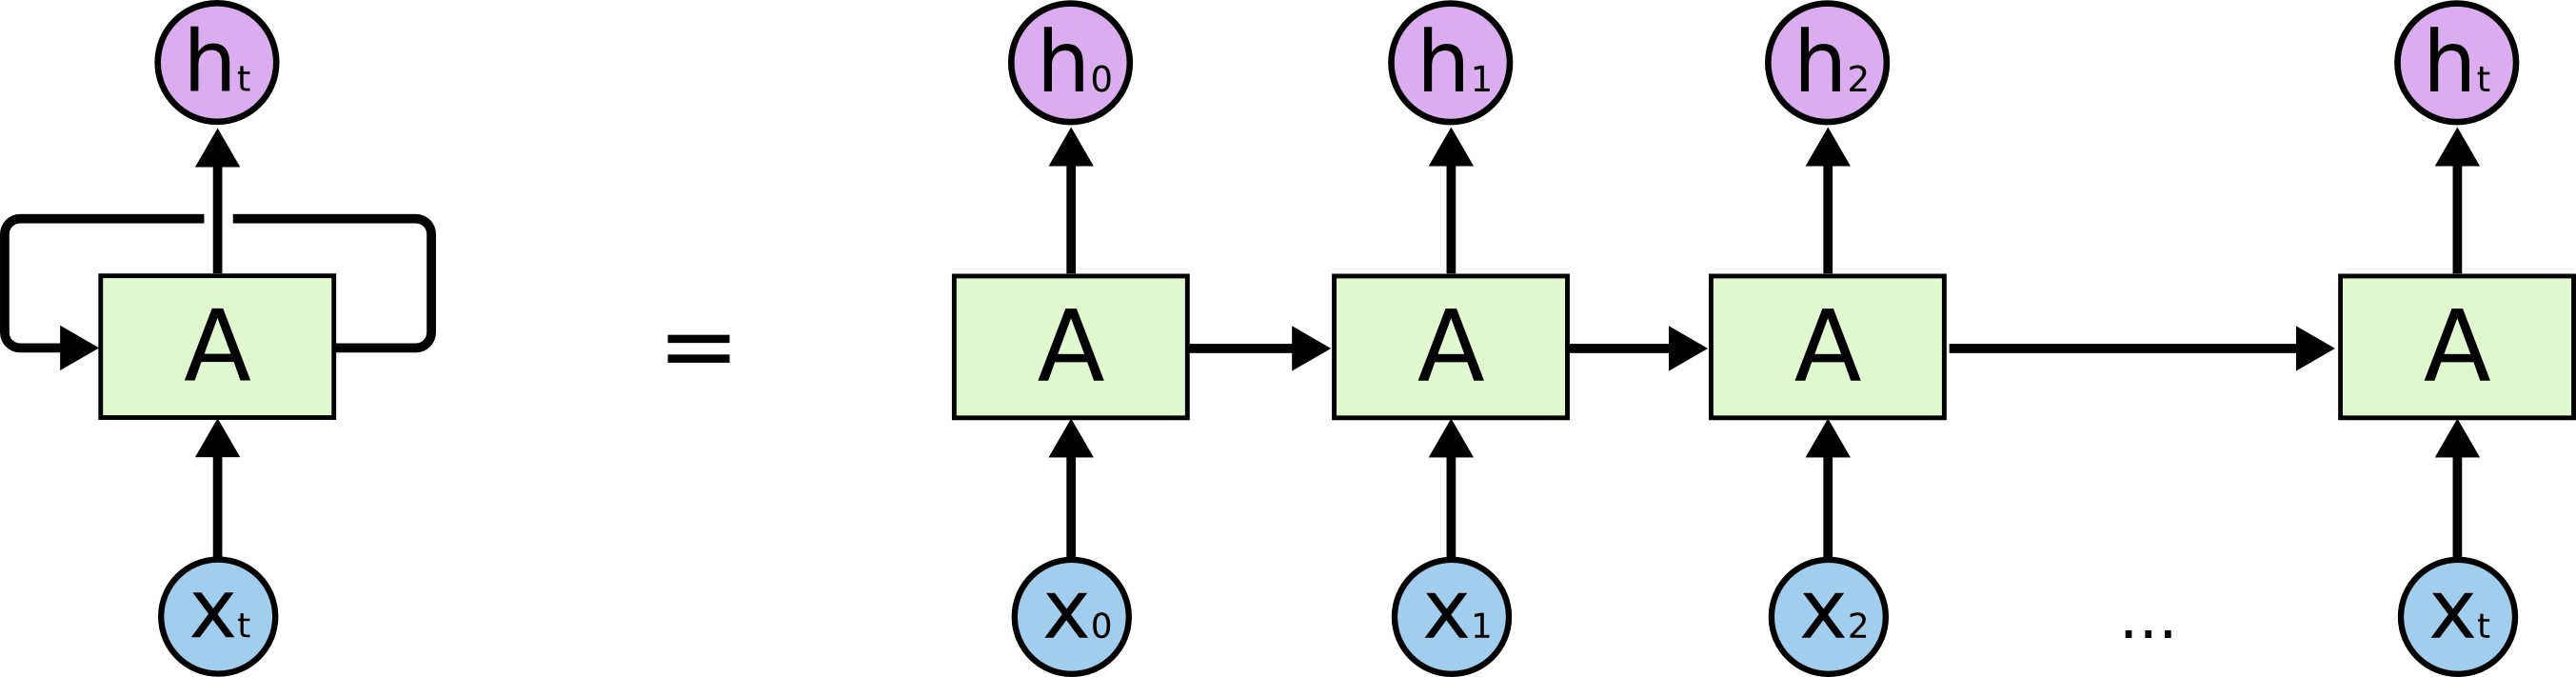
\includegraphics[width=0.9\textwidth]{fig/RNN-unrolled.png}
	\caption{Unrolling of the recurrent neural net.\cite{colah-lstm}
		\label{fig:rnn-unroll}}
\end{figure}
%reference http://colah.github.io/posts/2015-08-Understanding-LSTMs/

We can understand recurrent neural networks as very deep forward nets with shared weights. It is called RNN unrolling and it is described in figure \ref{fig:rnn-unroll}. Layers of this very deep net spread in time, together with the input sequence. This is very innovative idea, which enabled training RNN with backpropagation through time. It also shows that, as very deep networks, they have vanishing or exploding gradient problem, which means that the network is not able to learn long-term dependencies, even though in theory it should. This is a serious issue, which is caused by iterating many times over the weights and the activation function with derivatives $>1$ (exploding gradient) or $<1$ (vanishing gradient). Gradient then dies out and learning stops for distant dependencies. Among others this problem has been solved by the LSTM unit described in part \ref{subsec:lstm}, which is most popular now and following research resulting in GRU described in part \ref{subsec:gru}.

		\subsection{LSTM -- Long Short-Term Memory}\label{subsec:lstm}

Long Short-Term Memory nets are special kind of recurrent network, capable of learning long-term dependencies. This architecture was introduced by Hochreiter \& Schmidhuber\cite{Hochreiter:1997:LSM:1246443.1246450} after prior research of vanishing gradient problem\cite{hochreiter1991untersuchungen}. Later architecture was refined and popularized by other researchers\cite{DBLP:conf/ijcnn/GersS00,DBLP:journals/neco/GersSC00} and nowadays LSTM is most popular RNN architecture used.

The LSTM unit was designed to remember a value for an arbitrary length of time. It contains gates that determine when the input is significant enough to remember, when it should keep or forget the value, and when it should output the value. To understand the flow of data, see the diagram of a simplified LSTM unit on the figure \ref{fig:lstm}. All the gates can be described by the following series of equations.

%\begin{figure}[!ht]
%	\centering
%	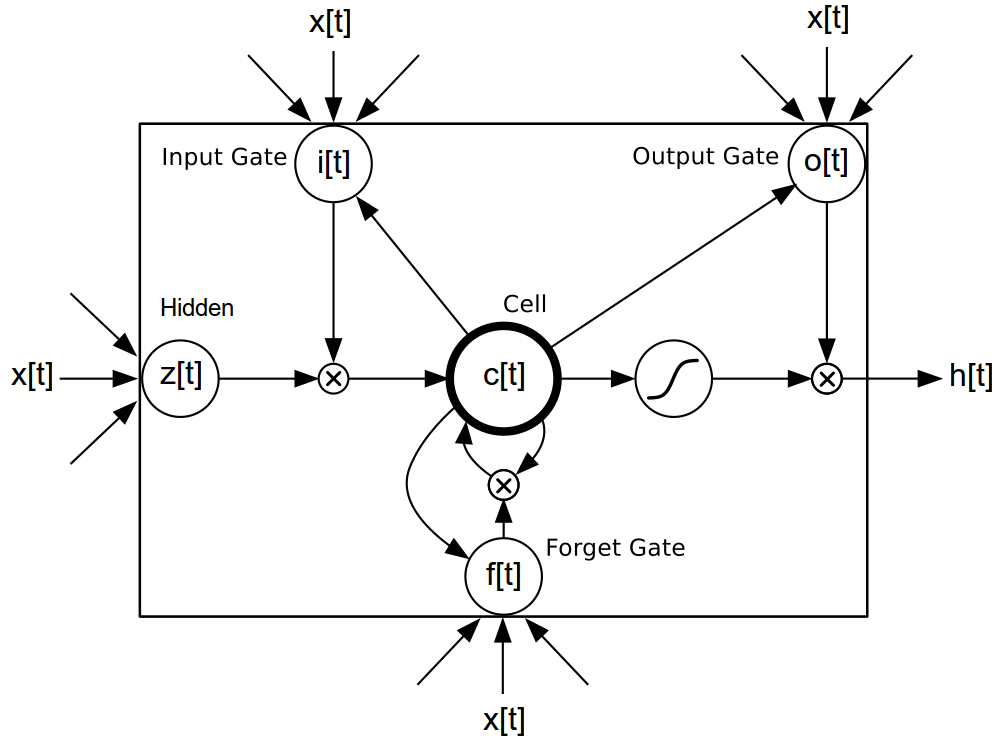
\includegraphics[width=0.7\textwidth]{./fig/LSTM-equations.png}
%	\caption{LSTM unit for equations
%		\label{fig:lstm-equations}}
%\end{figure}
\begin{figure}[!ht]
	\centering
	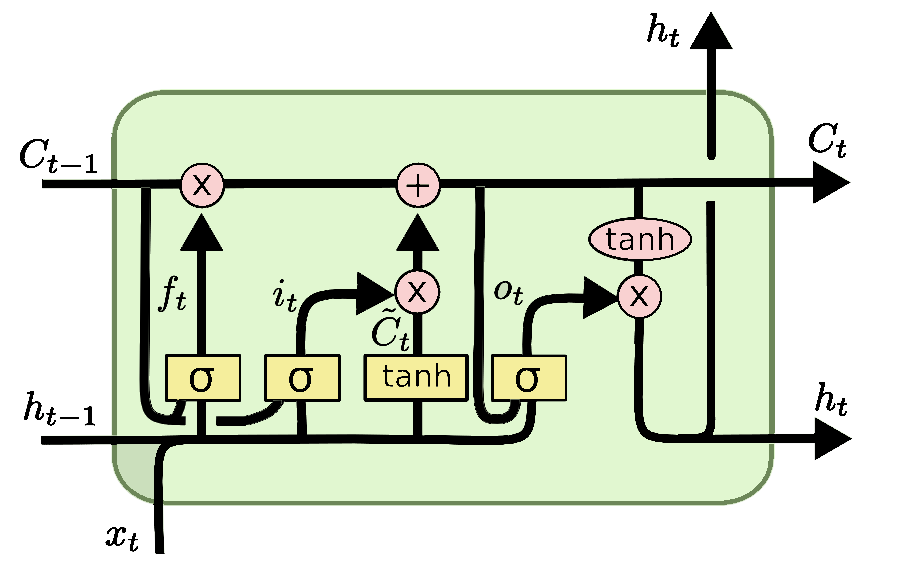
\includegraphics[width=0.7\textwidth]{./fig/LSTM3-var-peepholes.png}
	\caption{Variation of the LSTM unit.\cite{colah-lstm}
		\label{fig:lstm}}
\end{figure}
%reference http://colah.github.io/posts/2015-08-Understanding-LSTMs/

\belowdisplayskip=24pt
\begin{align}
	i_t \hspace{7pt}&=\hspace{7pt} \sigma(W_{xi}x_t + W_{hi}h_{t-1} + W_{ci}c_{t-1} + b_i) \label{eq:lstm1}\\
	f_t \hspace{7pt}&=\hspace{7pt} \sigma(W_{xf}x_t + W_{hf}h_{t-1} + W_{cf}c_{t-1} + b_f) \label{eq:lstm2}\\
	c_t \hspace{7pt}&=\hspace{7pt} f_t\odot c_{t-1} + i_t\odot \tanh(W_{xc}x_t + W_{hc}h_{t-1} + b_c) \label{eq:lstm3}\\
	o_t \hspace{7pt}&=\hspace{7pt} \sigma(W_{xo}x_t + W_{ho}h_{t-1} + W_{co}c_t + b_o) \label{eq:lstm4}\\
	h_t \hspace{7pt}&=\hspace{7pt} o_t\odot \tanh(c_t) \label{eq:lstm5}\\[16pt]
	\sigma(x) \hspace{7pt}&=\hspace{7pt} \frac{1}{1+e^{-x}} \label{eq:lstm7}
\end{align}

In each time slice the unit is using current input $ x_t $, last stored value $ c_{t-1} $ and unit output $ h_{t-1} $ to compute next state $ c_t $ and output $ h_t $. Variables $ i_t $, $ f_t $, $ o_t $ denotes value of input, forget and output gates which are used to control the information flow.

LSTM based on these equations is using total of 11 weight matrices and 4 bias vectors for computations and sigmoid function $ \sigma $ defined in the equation \eqref{eq:lstm7} and the operation $ \odot $ denotes the element-wise vector product. Equations described in this work are not the only way how to create an LSTM unit, but they will be used later while implementing the proposed model. Some of the versions are omitting \textquotedblleft peephole connections\textquotedblright, which allows gates to look at stored value $ C_{t-1} $, $ C_t $ or include only some of them.

Training of the LSTM based network can be performed effectively by standard methods like stochastic gradient descend in the form of backpropagation through time. Major problem with vanishing gradients during training described earlier is not an issue as backpropagated error is fed back to each of the gates.


		\subsection{GRU -- Gated Recurrent Unit}\label{subsec:gru}
Gated Recurrent Unit\cite{DBLP:journals/corr/ChoMGBSB14} is slightly more dramatic variation on the LSTM theme. It combines hidden state of the unit $ h_t $ with the saved value $ C_t $, merges input and forget gates into one update gate and removes peephole connections. These changes are simplifying standard LSTM models, but not at the expense of performance, and cause rapid growth in popularity. Diagram of the GRU unit is on the figure \ref{fig:gru}.

\begin{figure}[!ht]
	\centering
	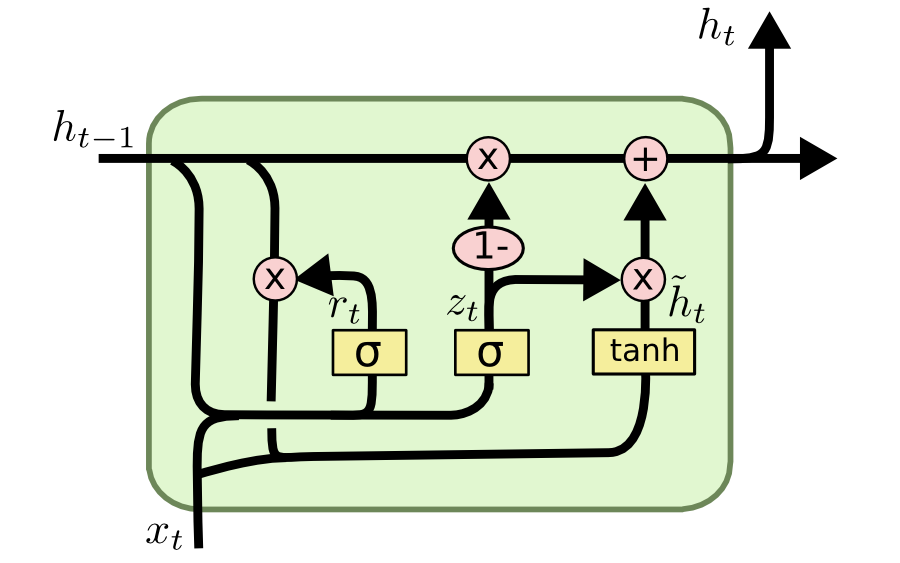
\includegraphics[width=0.7\textwidth]{./fig/LSTM3-var-GRU.png}
	\caption{Variation of a GRU unit.\cite{colah-lstm}
		\label{fig:gru}}
\end{figure}
%reference http://colah.github.io/posts/2015-08-Understanding-LSTMs/

\begin{align}
r_t \hspace{7pt}&=\hspace{7pt} \sigma(W_{xr}x_t + W_{hr}h_{t-1} + b_r) \label{eq:gru1}\\
z_t \hspace{7pt}&=\hspace{7pt} \sigma(W_{xz}x_t + W_{hz}h_{t-1} + b_z) \label{eq:gru2}\\
\widetilde{h}_t \hspace{7pt}&=\hspace{7pt} \tanh(W_{xh}x_t + W_{hh}(h_{t-1}\odot r_t) + b_h) \label{eq:gru3}\\
h_t \hspace{7pt}&=\hspace{7pt} (1-z_t)\odot \widetilde{h}_t + z_t\odot h_{t-1} \label{eq:gru4}\\[16pt]
\sigma(x) \hspace{7pt}&=\hspace{7pt} \frac{1}{1+e^{-x}} \label{eq:gru5}
\end{align}

Equations describe a version of GRU unit used in this work, with sigmoid function $ \sigma $ defined in equation \eqref{eq:gru5}. The operation $ \odot $ again denotes the element-wise vector product. While it is using only 4 weight matrices, 3 biases and just 1 state variable, researchers studied whether this can achieve at least same performance as previous LSTM unit.

Last year, study by Chung\cite{DBLP:journals/corr/ChungGCB14} was done, where different types of recurrent units were compared on the polyphonic music datasets. In this task LSTM and GRU were significantly better than all the other architectures, with GRU slightly in the lead. Generally, researchers agree that most of the LSTM variations, including GRU, are roughly on the same performance level. According to \cite{DBLP:journals/corr/GreffSKSS15} GRU is an average variation, slightly better than vanilla LSTM, with much simpler architecture.

In paper \cite{DBLP:conf/icml/JozefowiczZS15}, which emphasized variety of tasks and the data, GRU outperformed LSTM unit on all tasks with the exception of language modeling. There are multiple approaches to model languages and in this work I will explore different type than the one mentioned in Jozefowicz's paper\cite{DBLP:conf/icml/JozefowiczZS15}. More will be explained in following chapters. Interestingly they also found that LSTM nearly matched the GRU's performance, when its forget gate bias was initialized to 1 and not to naive initialization around 0.
It is also worth mentioning that Jozefowicz in his paper discovered several architectures similar to GRU, but with slightly better general performance. They were found by evolutionary algorithm working on candidate architectures  represented by the computational graph.


		\subsection{Language modeling and word embeddings}\label{subsec:lmAndEmbedd}

With the addition of LSTM units, recurrent neural nets quickly showed good performance in many different types of sequence processing like speech recognition from sound waves, signal prediction and language modeling. These result were further improved when researchers started stacking LSTMs on top of each other like pancakes.

Text is represented by discrete values and is usually presented to network in form of input vectors with one-hot encoding\footnote{One-hot encoded vector has exactly one high ('1') value and all the others low ('0').}. If we have a task with $ K $ classes, class $ i $ will be represented by a vector $ V $ of length $ K $. All the values of $ V $ will be switched off to 0, except $ V_i $, which will be 1. Vector $ V $ is simultaneously a degenerated multinomial probability distribution of the current input. If the output has the same shape as input, it can be simply created by softmax function at the output layer. Result will be proper multinomial distribution of next value, given current value.
% TODO \todof{pridat ukazky vektoru a pravdepodobnostniho rozlozeni}

At this point it is necessary to decide what will classes and defined vectors represent. In most cases, text prediction is performed at the word level. $ K $ is hence the number of words in the dictionary. This can cause some problems, as in bigger tasks dictionary often exceeds 100 000 records. This many classes require huge amount of training data to properly cover all the cases and high computational cost of the softmax layer is also an issue. This text representation cannot be used for texts not containing separate words, like multi-digit numbers. Nevertheless, state-of-the-art models have been using word-level representation. One of the advantages is no need to teach the net proper forms of the words. The net does not have to remember, how to spell the words properly and can learn other, more useful, features.

To solve the problem with extremely long input vectors, set of techniques called \emph{word embedding} were developed. They map words from the vocabulary to suitable vectors of real numbers in high dimensional space (around 50--1000 dimensions). Chosen vectors cannot be random, they are meaningful in order of performing some following task. For example Skip-gram model\cite{DBLP:journals/corr/abs-1301-3781} mapped 783 millions words to vectors of 300 real numbers, while creating reasonable relationships between them.
% TODO \todof{embedding - vice rozebrat, klidne s ukazkama na celou stranku}

%http://colah.github.io/posts/2014-07-NLP-RNNs-Representations/
%https://www.gavagai.se/blog/2015/09/30/a-brief-history-of-word-embeddings/

Character level modeling has been considered and used as an alternative to word-level, but so far had slightly worse performance. Regardless, it is still considered as an option, because it has much simpler representation of input and output. Consider roughly $ 45 $ characters in English text and over $ 50 000 $ words created from them. Character level network is also more suited for Czech or Russian and other fusional\footnote{Fusional language is a type of language distinguished by its tendency to overlay many morphemes to denote grammatical, syntactic, or semantic change.} languages, which heavily use prefixes and suffixes to create new words. This is also an ability, which cannot be overlooked, as it is not available for word level.
Character level models have usually smaller vocabulary size and have to be trained longer, as they need to learn spelling of the words on top of the same features of word level. With the properly trained character level model we can benefit from its much greater generative abilities, than we can achieve with word-level.

	\section{Convolutional neural nets}
	
Feed-forward neural nets together with backpropagation algorithm showed very useful for range of tasks and it has even been proven\cite{cybenko:mcss,journals/nn/Hornik91} they can approximate any continuous function. However, they were not very good in recognizing objects presented visually. As every unit is connected to large amount of units in the next layer (or all of them in fully-connected layers), the number of weights grows rapidly with the size of the problem and even more with the dimensionality. All these problems are manifesting even in image processing with only two dimensions. Convolutional neural nets (CNN) were introduced as a solution to reduce the number of parameters involved, while exploiting spatial constraints in the input.

Ideas of convolutional nets took inspiration from neurobiology, more precisely from the organisation of neurons in visual cortex of the cat. They were first used in the work of Homma\cite{NIPS1987_20} to process temporal signal. Later their design was improved by LeCun et al. \cite{lecun-98}. Different CNN architecture was proposed by Graupe\cite{graupe1988} for decomposition of one-dimensional EMG signals. Convolutional nets can be also used to natural language processing\cite{DBLP:journals/corr/Kim14f} and to analysis of three-dimensional data like videos\cite{10.1109/TPAMI.2012.59} or volumetric data (eg. 3D medical scans), but that is not as common as image processing.

Basic architecture of CNN can be described as the following process:

\vspace{8mm}
\begin{minipage}{0.9\textwidth}
\begin{enumerate}
	\item Convolve several small filters on the input.
	\item Subsample this space of filter activations.
	\item Repeat steps 1 and 2 until you are left with a sufficiently high level features.
	\item Use a standard feed-forward neural net to solve the task, using the features as input.
\end{enumerate}
\end{minipage}
\vspace{1cm}

Convolutional layer, which is most important and gave CNN their name is essentially the same as mathematical convolution used elsewhere. Here it means to apply a 'filter' over an input at all possible offsets. This filter - in image processing and computer vision called kernel - has a layer of connection weights with the same dimensionality as the input, but with much smaller size. Despite the fact that there is many connections, which are even overlapping, the weights are tied together and during training only handful of parameters per filter need to be updated. It is also possible to stack filters on top of each other to create more powerful architectures, but as they do not reduce dimensionality significantly, output has the same size as the input. Second type of a layer has been introduced to improve it - subsampling.

Subsampling, or max pooling in this version, is a simple operation that takes small non-overlapping grid of the input tensor and outputs the maximum value of each part. By putting this operation in between the convolutional layers, we can detect higher level features than without it.

Last type of unit commonly used in CNN is rectified linear unit (ReLU), which provides nonlinearity and improves overall performance\cite{jarrett-iccv-09,icml2010_NairH10}. One of the first and most famous examples of convolutional neural net is LeNet\footnote{Demos and examples of LeNet: \url{http://yann.lecun.com/exdb/lenet/}}\cite{lecun-98}, which recognize handwritten digits from the MNIST database\footnote{MNIST database website: \url{http://yann.lecun.com/exdb/mnist/}}. Architecture of LeNet-5 is on the figure \ref{fig:lenet}.

\begin{figure}
	\centering
	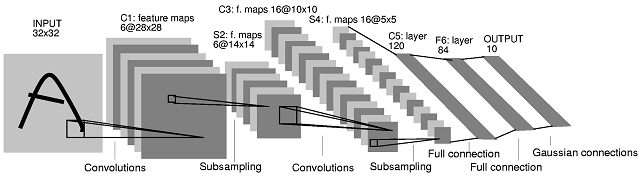
\includegraphics[width=\textwidth]{./fig/lenet-architecture.png}
	\caption{LeNet-5 architecture.\cite{lecun-98}
		\label{fig:lenet}}
\end{figure}

\chapter{Image caption generation}\label{chp:captions}

Scene understanding is one of the fundamental and most difficult tasks of computer vision. Being able to automatically generate image or video captions in regular text could have great effect. However, it is much more complicated than simple classification or object recognition, because the model also need to understand relations between the recognized objects and capture that correctly in the captions.

In this chapter I will do an overview of approaches to this task and more closely describe latest papers on which is this work based (section \ref{sec:related}). Following parts cover datasets (\ref{sec:datasets}) and evaluation procedures (\ref{sec:evaluation}) most commonly used for this task.

	\section{Related Work}
	\label{sec:related}
	
Currently, neural networks are most heavily used to generate captions. Before them two main approaches were common. The first one used caption templates, which were filled by detected objects and relations. Second was based on retrieving similar captions from database and modifying them to fit current image. Question of similarity ranking has been addressed by many papers, which are based on the idea of joint embedding vector space for both images and captions\cite{DBLP:journals/corr/KarpathyF14}. Similar descriptions are in this space close to each other.

Both approaches above usually included generalization step to remove information relevant only to current image, for example names. They are quite successful in describing images, but they are heavily hand-designed and their text-generation power is fixed on the database/embedding and is not able to describe previously unseen compositions of objects. Over time these approaches fell out of favor to now dominant neural network methods.

Many of the methods using neural nets are inspired by successes in training of recurrent nets for machine translation. It is worth mentioning Sutskevers work \cite{DBLP:journals/corr/SutskeverVL14}, which studied general sequence to sequence mapping by converting input sequence to vector of fixed length. Vector is then decoded to output sequence. This encoder--decoder architecture is closely related to autoencoders and work of Kalchbrenner and Blunsom\cite{conf/emnlp/KalchbrennerB13}, who were first to map the entire input sequence to vector.

The introduced encoder--decoder architecture is important to the captioning task, because we can interpret image description problem as a translation from an image to a sentence. In this case, encoder part of the model is usually convolutional neural net, as they are excellent in the image classification\cite{DBLP:journals/corr/SzegedyLJSRAEVR14}. Decoder part is similar as in machine translation models -- type of a RNN or LSTM, as the output for both tasks is essentially same.

One of the most interesting event in this field is MS COCO Captioning Challenge\footnote{MS COCO Challenge: \url{http://mscoco.org/dataset/\#captions-challenge2015}} in which many of the state-of-the-art researchers compete directly against each other. Most of the works described further have participated in this challenge.

%\todo[inline]{nejlepsi clanky se ucastni ms coco.}

		\subsection{Show and Tell: A Neural Image Caption Generator} \label{subsec:showtell}
		
Model from this paper\cite{DBLP:journals/corr/VinyalsTBE14}, made by Google researchers, tied for the first place in MS COCO Captioning Challenge with the following Microsoft model \ref{subsec:fromCaptions}. The main idea for this work is to use recent advancements in machine translation and apply them for image captioning. Model uses encoder--decoder architecture, with CNN for the encoder part and RNN for the decoder part, as described earlier, which is trained to maximize the likelihood $ p(S|I) $ of producing a target sequence of words $ S = \{S_1,S_2,...\} $ given an input image $ I $.
		
Used convolutional neural net has been pre-trained for an image classification task and last hidden layer of this network has been used as an input to the RNN decoder that generates word sequences. The decoder part of the network is made of LSTM units based on the following equations:

\belowdisplayskip=24pt
\begin{align}
i_t \hspace{7pt}&=\hspace{7pt} \sigma(W_{xi}x_t + W_{hi}h_{t-1}) \label{eq:showlstm1}\\
f_t \hspace{7pt}&=\hspace{7pt} \sigma(W_{xf}x_t + W_{hf}h_{t-1}) \label{eq:showlstm2}\\
o_t \hspace{7pt}&=\hspace{7pt} \sigma(W_{xo}x_t + W_{ho}h_{t-1}) \label{eq:showlstm3}\\
c_t \hspace{7pt}&=\hspace{7pt} f_t\odot c_{t-1} + i_t\odot\tanh(W_{xc}x_t + W_{hc}h_{t-1}) \label{eq:showlstm4}\\
h_t \hspace{7pt}&=\hspace{7pt} o_t\odot c_t \label{eq:showlstm5}
\end{align}
		
Notation is same as in the chapter \ref{chp:nn}, $ \sigma $ is the sigmoid function and the operation $ \odot $ denotes the element-wise vector product.

\begin{figure}[!ht]
	\centering
	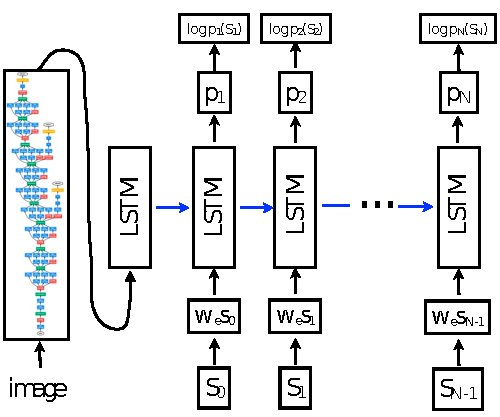
\includegraphics[width=0.4\textwidth]{./fig/show-tell_model.pdf}
	\caption{\textquoteleft Show and Tell\textquoteright\ image captioning model.\cite{DBLP:journals/corr/VinyalsTBE14}
		\label{fig:showmodel}}
\end{figure}

RNN produces output on the word level, using word embedding vectors\cite{DBLP:journals/corr/abs-1301-3781}, one at a time. Complete procedure and architecture of the model with the unrolled RNN, word embeddings and \emph{softmax} layer is on the figure \ref{fig:showmodel}. Computing procedure of the model equal to the image is on the following equations:

\belowdisplayskip=24pt
\begin{align}
x_{-1}  \hspace{7pt}&=\hspace{7pt} CNN(I) \label{eq:showmodel1}\\
x_t     \hspace{7pt}&=\hspace{7pt} W_eS_t,\hspace{15pt} t\in\{0\ldots N-1\}  \label{eq:showmodel2}\\
p_{t+1} \hspace{7pt}&=\hspace{7pt} LSTM(x_t),\hspace{15pt} t\in\{0\ldots N-1\}  \label{eq:showmodel3}
\end{align}		
		
Each word is represented as a one-hot vector $ S_t $ of the size equal to size of the dictionary. Special start word $ S_0 $ and stop word $ S_N $ designated to mark start and end of the sequence are also present. Both the image and the words are mapped to the same space. Input image embedding is fed to the LSTM only once, at $ t=-1 $.
		
The CNN component of the model has been initialized to an ImageNet trained model, which helped quite a lot in terms of generalization. Word embeddings were left uninitialized (initialized randomly) as they did not observed significant gains while using large corpus. Dropout and ensebling used during training gave minor improvements. Model has been trained using stochastic gradient descent with fixed learning rate and no momentum. For the embeddings and the LSTM memory 512 dimensions were used. During the inference, beam search has been used to improve the results.
				
		\subsection{From Captions to Visual Concepts and Back} \label{subsec:fromCaptions}
		
This paper\cite{DBLP:journals/corr/FangGISDDGHMPZZ14} took quite a different approach than a previous one, however both tied for the first place in the competition. This model is not end-to-end, it has three stages. First, it learns to extract nouns, verbs and adjectives from regions in the image. These words come from the vocabulary constructed by using 1000 most common words in the training captions. By running detector on the image regions, model is able to produce bag of bounding boxes. Each bounding box represent location of word in the image. Network pretrained on ImageNet is used for initialization.

Second, these extracted words guide a language model to generate text, which include these words. The maximum entropy (ME) language model estimates the probability of a word $ w_i $ conditioned on the preceding words, as well the words with high likelihood detections, yet to be mentioned. This encourages all the words to be used, while avoiding repetitions. A left-to-right beam search similar to \cite{DBLP:journals/corr/cs-CL-0006028} is used during generation. After extending each sentence with a set of likely words, the top $ N $  sentences are retained and the others pruned away. The process continues until a maximum sentence length $ L $ is reached.

Third, candidate captions are re-ranked using MERT\cite{och2003minimum} (Minimum Error Rate Training) and the best one is selected. MERT uses linear combination of features computed over the sentence, for example log-likelihood of the sequence or its length. One of the features is Deep Multimodal Similarity Model (DMSM) score, which measures similarity between images and text. The DMSM is model proposed in this paper, which learns two neural networks that map images and text fragments to a common vector representation. These vectors are used to compute the cosine similarity score, which is one of the features fed to MERT.

Direct comparison of this approach with the first one, presented in the paper description \ref{subsec:showtell}, is in paper \cite{DBLP:journals/corr/DevlinCFGDHZM15} by the same authors. They examine the issues of both approaches and achieve state-of-the-art performance by combining key aspects of RNN and ME methods.
		
		\subsection{Show, Attend and Tell: Neural Image Caption Generation with Visual Attention}
	
Work \cite{DBLP:journals/corr/XuBKCCSZB15} of researchers from universities in Toronto and Montreal was inspired by recent work in machine translation and introduced an attention based model. Attention is one of the most interesting parts of the human visual system. Rather than compressing an entire image into a static representation, attention allows for salient features to dynamically come to the forefront as needed. Proposed model has encoder-decoder architecture. Encoder part use a convolutional neural network to extract set of feature/annotation vectors (not just one). Each of the vectors correspond to a part of image. Features from a lower convolutional layer are used to obtain a correspondence between them.

Decoder part is a LSTM network working of the word level, which generates, apart from the word of the output, a context vector - a dynamic representation of the relevant part of the image at time $ t $. The paper explored two attention mechanisms computing the context vector from the annotation vectors. First is the stochastic \textquotedblleft hard\textquotedblright\ mechanism, which interprets the values in the context vector as the probability that corresponding location is the right place to focus for producing the next word. Second is deterministic \textquotedblleft soft\textquotedblright\ mechanism introduced in \cite{DBLP:journals/corr/BahdanauCB14}. Which gives the relative importance of the location by blending values for all annotation vectors together. This method is fully trainable by standard back-propagation methods.

\begin{figure}[!ht]
	\centering
	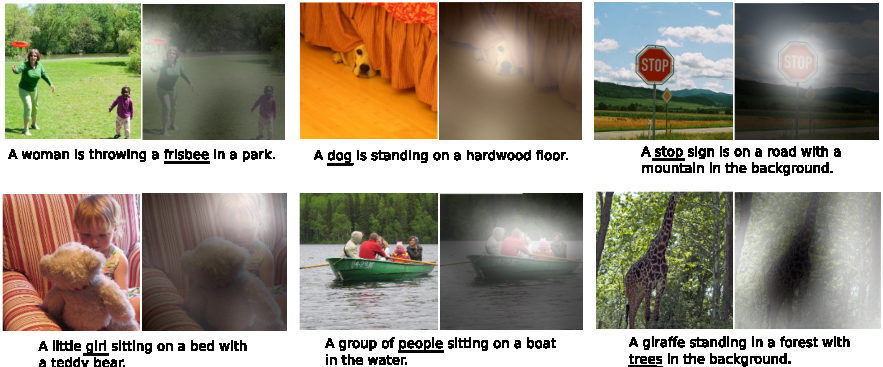
\includegraphics[width=0.95\textwidth]{./fig/show-attend-tell_example-correct.pdf}
	\caption{Examples of attending the correct object while generating the word.\cite{DBLP:journals/corr/XuBKCCSZB15}
		\label{fig:attendmodelcorrect}}
\end{figure}

\begin{figure}[!ht]
	\centering
	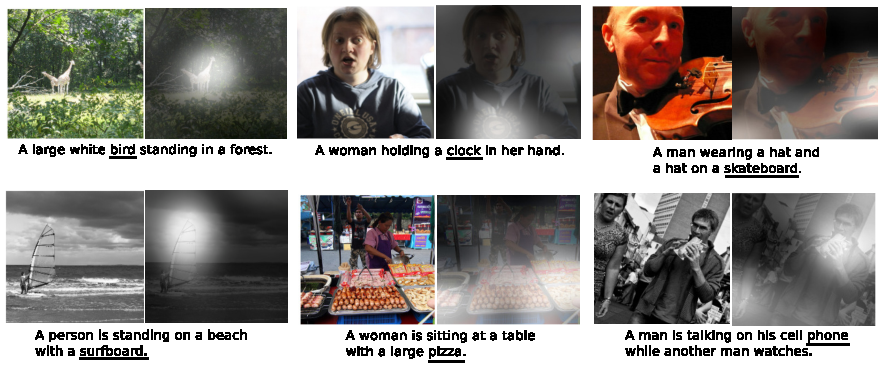
\includegraphics[width=0.95\textwidth]{./fig/show-attend-tell_example-wrong.pdf}
	\caption{We can use attention to understand what the model saw while creating wrong caption.\cite{DBLP:journals/corr/XuBKCCSZB15}
		\label{fig:attendmodelwrong}}
\end{figure}

Paper is also showing how we can gain insight and interpret the results of the model by visualising where and what the attention was focused on. Examples of the correct visualisations is on the figure \ref{fig:attendmodelcorrect} and the wrong ones on the figure \ref{fig:attendmodelwrong}. Visualisations show that model can attend even \textquotedblleft non-object\textquotedblright\ regions. This adds an extra layer of interpretability to the output. The model learns alignments that correspond very strongly with human intuition. Especially in the examples of mistakes, we can understand why those mistakes were made.

CNN trained on ImageNet without finetuning was used for the decoder part. Model was trained with several algorithms and researchers found that for Flickr8k dataset, RMSProp worked best, while for Flickr30k and MSCOCO datasets, Adam\cite{DBLP:journals/corr/KingmaB14} algorithm was used. Performance during training was also improved by creating minibatches of sentences with same length, which greatly improved convergence speed.
		
		\subsection{Long-term Recurrent Convolutional Networks for Visual Recognition and Description}

The research group from Berkeley in paper \cite{DBLP:journals/corr/DonahueHGRVSD14} presented long-term recurrent convolutional network (LRCN), which combines convolutional and long-range temporal layers for several tasks. It is possible to apply the introduced network to recognize activity performed on the video (sequential input $ \mapsto $ fixed output), generate description  of the image (fixed input $ \mapsto $ sequential output) or describe video (sequential input $ \mapsto $ sequential output). 

Architecture of the proposed model is similar to the one from part \ref{subsec:showtell}, only output of the CNN is fed to the LSTM in each time step. According to the task specification model can use separate convolutional networks, different for each time step, each with specific input or single CNN through all the time steps. Example is on the figure \ref{fig:LRCN}.

\begin{figure}[!ht]
	\centering
	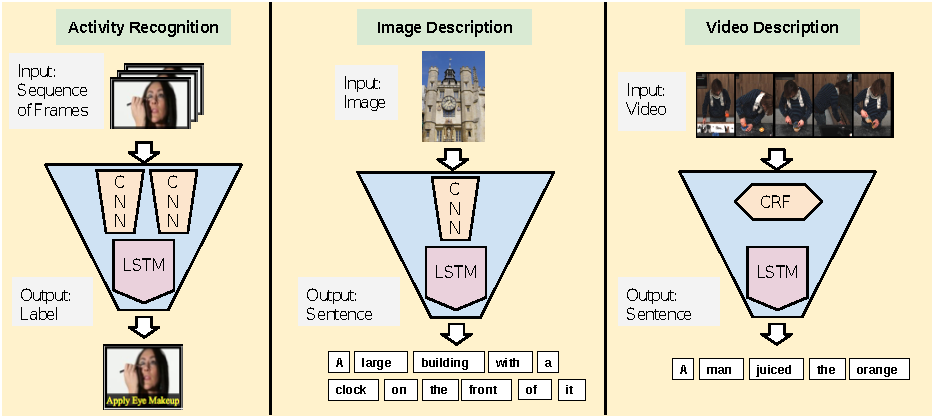
\includegraphics[width=0.95\textwidth]{./fig/long-term-rec-con.pdf}
	\caption{Task-specific instantiations of the LRCN model.\cite{DBLP:journals/corr/DonahueHGRVSD14}
		\label{fig:LRCN}}
\end{figure}

	\section{Datasets}
	\label{sec:datasets}		
Big datasets are necessary requirement in training recurrent neural nets, together with sufficient computing power. As access to machines and hardware suitable for training has been made extremely easy, obtaining enough data become the biggest problem. All the descriptions in the image captioning datasets have to be human generated, which is very expensive. This is one of the reasons, not many specialized datasets are created.

There are two main options how to get images and captions. First, using user-generated data from an online service, most commonly Flicker. However, captions are not made specifically for the task and could be prone to error. Second option is to create captions directly for use in the dataset. Amazon Mechanical Turk\footnote{Amazon Mechanical Turk is crowdsourced Internet marketplace to perform tasks that computers are currently unable to do.} is heavily used for this task. All datasets mentioned here are created this way.

Flickr8k\cite{dataset-flickr8k} was one of the first datasets created for this purpose. It has been later expanded into Flickr30k\cite{dataset-flickr30k}. MS COCO\cite{DBLP:journals/corr/ChenFLVGDZ15} is dataset created by Microsoft for their captioning challenge. CIDEr\cite{Vedantam_2015_CVPR} datasets PASCAL-50S, ABSTRACT-50S are youngest mentioned, designed specifically for evaluation with the CIDEr metric.

\def\arraystretch{1.2}%  1 is the default, change whatever you need
%\setlength\extrarowheight{20pt}%add points to the row height

\begin{center}
	\begin{longtable}{|l|m{2cm}|m{2cm}|m{4.7cm}|}			
		\caption{Image captioning datasets.} \label{tab:datasets} \\

	   	\hline
	   	\multicolumn{1}{|l|}{\textbf{Name}} & 
	   	\textbf{Images} & 
	   	\textbf{Captions per image} & 
	   	\textbf{Note} \\
	   	\hline \hline
		\endhead
		
	   	Flickr8k\footnote{Flickr8k project: \url{http://nlp.cs.illinois.edu/HockenmaierGroup/8k-pictures.html}} &
		   	\multicolumn{1}{r|}{8 092} &
		   	\multicolumn{1}{c|}{5} &
		   	Focused on people or animals (mainly dogs) performing some specific action. \\ \hline
	   	Flickr30k\footnote{Flickr30k project: \url{http://shannon.cs.illinois.edu/DenotationGraph/}} & 
		   	\multicolumn{1}{r|}{31 783} &
		   	\multicolumn{1}{c|}{5-6} &
		   	An extension of Flickr8k dataset. \\ \hline
	   	MS COCO\footnote{MS COCO project: \url{http://mscoco.org/dataset/}} &
		   	\multicolumn{1}{r|}{120 000} &
		   	\multicolumn{1}{c|}{5} &
		   	Images are divided - 80 000 for training and 40 000 for testing purposes. \\ \hline
	   	PASCAL-50S\footnote{\label{ft:cider}PASCAL-50S and ABSTRACT-50S: \url{http://ramakrishnavedantam928.github.io/cider/}} &
		   	\multicolumn{1}{r|}{1 000} &
		   	\multicolumn{1}{c|}{50} &
		   	Built upon images from the UIUC Pascal Sentence Dataset. \\ \hline
	   	ABSTRACT-50S\footnote{See footnote \ref{ft:cider}.} &
		   	\multicolumn{1}{r|}{500} &
		   	\multicolumn{1}{c|}{50} &
		   	Built upon images from the Abstract Scenes Dataset. No photos.\\ \hline
	\end{longtable}
\end{center}

	\section{Evaluation}
	\label{sec:evaluation}	
Recent progress in fields like machine translation, which are very similar to image captioning, caused spike of interest in evaluating regular text output accuracy. Although it is sometimes not clear if a description of an image is best option available, some degree of assessment is possible. The best results can be obtained by asking live raters to give a score on the usefulness of each description. Subjective scores can vary, but it can be averaged by giving same description to multiple raters. However this method consumes tremendous amount of time and usually external raters are necessary. Tools like Amazon Mechanical Turk can be used to great extent, but need for automated tools is evident.

		\subsection{Automated metrics}
		
Assuming that one has access to human generated captions, which is ground truth in our case, completely automated metrics exists. Even though all of them compute how alike are generated to human descriptions, different approaches are used. One metric can use several different settings with slight changes in the algorithm. This raises the question, how can we compare results of different works, despite using the \textquotedblleft same\textquotedblright \ evaluation method. Microsoft group of researchers addresses this issue in \cite{DBLP:journals/corr/ChenFLVGDZ15}. They created an evaluation server\footnote{MS COCO evaluation server: \url{http://mscoco.org/dataset/\#captions-upload}.} which has many automated metrics, with several configurations, including all mentioned here. It will serve as a reference point for comparing image captioning models.
		
The most commonly used metric has been BLEU (Bilingual Evaluation Understudy)\cite{Papineni:2002:BMA:1073083.1073135}, which was created in 2002 to evaluate quality of machine translated text from one language to another. Scores are computed on individual segments, usually sentences. BLEU has high correlation with human judgments and is still highly popular even for captioning tasks. However, it is becoming outdated as automatic methods are now outperforming humans. Four different variations of BLEU are used in MS COCO evaluation server.

METEOR (Metric for Evaluation of Translation with Explicit ORdering)\cite{Lavie:2007:MAM:1626355.1626389} is another metric for the evaluation of machine translation from 2007. It was designed to fix some problems of the BLEU metric and it can also look for synonyms and perform stemming on input words.
		
Last year, metric designed directly to caption evaluation called CIDEr (Consensus-based Image Description Evaluation)\cite{Vedantam_2015_CVPR} was introduced. This is still new metric, but with growing popularity as it correlate well with human judgment. Main idea of this metric is that given enough captions for the same image, metrics perform better. This can be seen in datasets introduced with it (see part \ref{sec:datasets}).		

\chapter{Tools and Experiments}\label{chp:exper}

In this chapter I will describe tools and frameworks, which are used to implement deep learning models. \emph{Torch} will be discussed separately in its own section as it was a tool I used for experimenting with language modeling - predicting next character in text, which is second part of this chapter.

%The landscape of tools for neural networks is changing rapidly, so please bear in mind that if you are reading this several years later, some of the information does not have to be valid anymore.

One of the tools most academic researchers in deep learning rely on is \emph{Theano}\footnote{Theano: \url{http://deeplearning.net/software/theano/}}\cite{bergstra-proc-scipy-2010}, which is Python library that works with mathematical expressions and matrices. It is built upon \emph{NumPy} to handle multidimensional arrays and compiles expressions before use for efficient computation. Theano can be quite intimidating and non-intuitive for some people, as it is focused on researchers and creating new architectures. For this reason, many packages and libraries has been created on top of Theano to simplify and streamline development of standard models. Among most popular are \emph{Keras}\footnote{Keras: \url{https://github.com/fchollet/keras}}, \emph{Lasagne}\footnote{Lasagne: \url{https://lasagne.readthedocs.org/en/latest/}}, \emph{Blocks}\footnote{Blocks: \url{https://github.com/mila-udem/blocks}}, which are open-source and available on GitHub, and \emph{PyLearn2}\footnote{PyLearn2: \url{http://deeplearning.net/software/pylearn2/}}.

Next Python library, independent of Theano, is \emph{TensorFlow}\footnote{TensorFlow: \url{https://www.tensorflow.org/}}, a tool from Google, released last year. It is used to process symbolic data flow graphs on many different types of machines, ranging from multiple GPU computers to smartphones. Interesting feature is ability to perform partial subgraph computation, which allows distributed training of the neural network. TensorBoard is a tool worth mentioning, as it provides visualisations of training and evaluation of the model, tool missing in most of the other libraries.

Python tools with the engine implemented in C/C++ are not the only ones. \emph{Caffe}\footnote{Caffe: \url{http://caffe.berkeleyvision.org/}} is well-known and widely used library with API in C++. It performs very well in image classification with neural nets and can be used as a source of many pre-trained models hosted on the Model Zoo\footnote{Caffe Model Zoo: \url{https://github.com/BVLC/caffe/wiki/Model-Zoo}} site. It is also possible to use \emph{Deeplearning4j}\footnote{Deeplearning4j: \url{http://deeplearning4j.org/}}, which is deep-learning library written for Java and Scala, and a lot of others. Nowadays, libraries are introduced almost every month as this field is very live, which also means not everything is implemented in every framework and users need to follow news about their tools.

\section{Torch}

\emph{Torch}\footnote{Torch: \url{http://torch.ch/}} is an open source scientific computing framework and machine learning library for the Lua. Underlying implementation is using extremely fast LuaJIT and C, but no need to code in C is required. Torch is not as popular in academic environment as Theano, but it is used by several large companies including Google \& DeepMind, Facebook and IBM, which also contribute to the project. Apart from the companies, Torch has a large ecosystem of community-driven packages\footnote{Wikipage with list of packages: \url{https://github.com/torch/torch7/wiki/Cheatsheet}} with almost every tool needed for machine learning, computer vision and signal processing, and wide range of utilities. In the rest of this section I will describe fundamental Torch packages, which are necessary for my research.

The core package of Torch is \emph{torch}, which is installed together with the library. It contains data structures for multi-dimensional tensors and operations over them. This is the most important part, as almost every package depends on them. Additionally, it provides many utilities for accessing files, serializing objects, processing command-line parameters and other useful utilities.

\subsection{nn, nngraph}

The base Torch provides necessary math structures, but the \emph{nn} package allows simple creation of neural networks with a common \texttt{Module} interface. Module represents a layer of the network, which is the building block of the nets in Torch. Layers have \texttt{forward()} and \texttt{backward()} method and can be joined together by module composites \texttt{Sequential}, \texttt{Parallel} and \texttt{Concat}. These components allows creation of arbitrary graphs.

The \emph{nn} package also contains loss functions, which are subclasses of \texttt{Criterion}. Classes \texttt{ClassNLLCriterion} and \texttt{CrossEntropyCriterion} contain common cross-entropy classification criterion. Other regression and embedding criterions are also available together with simple method to train the network with stochastic gradient descent.

Creating networks with complex graphs is quite complicated with the \emph{nn}. To make it easier, \emph{nngraph} package has been introduced. \emph{nngraph} bundles \emph{nn} modules into graph nodes, which are linked together by specifying inputs and outputs. Graphs can be visualized by \texttt{dot()} method and exported to vector graphics.

Both packages are sufficient and provide even advanced features like weight-sharing or weight-tying. They are mainly focused on feed-forward and convolutional networks. Creating RNNs is possible, however it is very complicated and labor-intensive.

\subsection{rnn}\label{subsec:torch-rnn}

Torch's \emph{rnn}\cite{DBLP:journals/corr/LeonardWW15} package extends \emph{nn} can be used to build recurrent neural nets, LSTM and GRU layers, and so on. The package handles the unrolling of a network and provides several options how to train a network. One of the ways is to use \texttt{backwardOnline()}, call \texttt{forward()} method repeatedly and then go \texttt{backward()} in the opposite order. Other option is to decorate model with \texttt{Sequencer} and feed the sequence to the network with only one \texttt{forward()} and one \texttt{backward()} call.

Package also provide module for implementing attention model\cite{DBLP:journals/corr/MnihHGK14}. It is worth mentioning that creating complex recurrent networks with the \emph{nngraph} package might be difficult, as both packages are altering \emph{nn} functionality and may collide.

\subsection{Other packages}

As the number of community packages is enormous, I will list just a few, which are commonly used and related to the topic of this work:

\vspace{5mm}
\begin{minipage}{0.9\textwidth}
	\begin{itemize}
		\item \emph{optim} --- Optimization library with SGD, AdaGrad, RMSProp and more.
		\item \emph{nninit} --- Weight initialisation schemes for nn modules
		\item \emph{image} --- Routines to load/save and manipulate images as \emph{torch} tensors.
		\item \emph{word2vec} --- Pre-trained word embeddings and the distance metric.
		\item \emph{cunn}, \emph{clnn} --- CUDA and OpenCL backends for \emph{nn} package.
		\item \emph{loadcaffe} --- Method for loading Caffe models in Torch.
	\end{itemize}
\end{minipage}
\vspace{3mm}

\section{Predicting next character in sequence}

As an application of the Torch library, I created a model predicting next character in a text, as described in part \ref{subsec:lmAndEmbedd}. Compilation of all Shakespeare's works have been used as an input data, as in Karpathy's post\cite{char-rnn}.

Models used one-hot encoding for the input and probability distribution of the next character in sequence as an output. Networks have three recurrent layers (LSTM or GRU), each with 400 nodes, followed by linear and logarithmic softmax layer. Architectures are on the images \ref{fig:chargen1} and \ref{fig:chargen2}.

\begin{figure}[htb]
	\begin{minipage}{.47\textwidth}
		\centering
		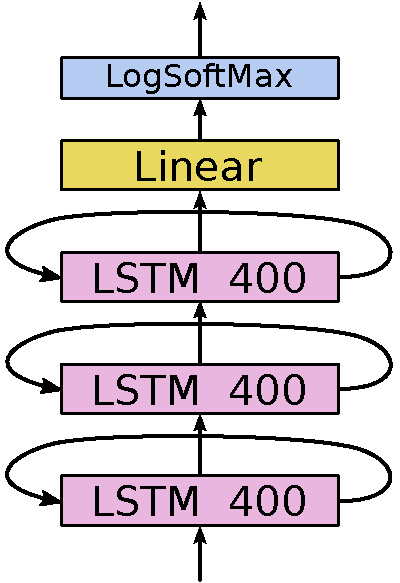
\includegraphics[width=0.7\textwidth]{./fig/char-rnn-model1.pdf}
		\caption{Architecture of the LSTM model.
			\label{fig:chargen1}}
	\end{minipage}
	\hfill
	\begin{minipage}{.47\textwidth}
		\centering
		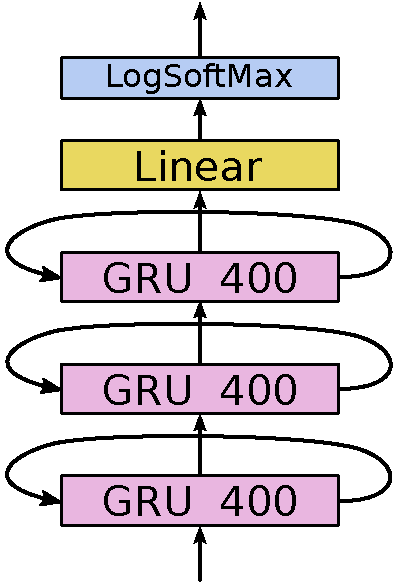
\includegraphics[width=0.7\textwidth]{./fig/char-rnn-model2.pdf}
		\caption{Architecture of the GRU model.
			\label{fig:chargen2}}
	\end{minipage}
\end{figure}

LSTM model was trained with stochastic gradient descent with Nesterov's momentum on minibatches of 20 subsequences, each with 40 characters. GRU model was trained with SGD without momentum, however, weight decay was used. After couple of hours, models were producing following samples:

\begin{center}
	\begin{longtable}{|l|m{11cm}|}					
		\caption{Predictions of the models.} \label{tab:predictions}\\

		\hline
		\textbf{Inicialization} &
		\begin{lstlisting}
And therefore has he closely mew'd her u
		\end{lstlisting}\\ \hline
		\textbf{LSTM model}&
		\begin{lstlisting}
ndon,
And, ine and Frenice handle and forth can hday for pu-chang but riothed.

QUEEN ELIZABETH:
Whyou art me yough to hell three,
?gecT blswance'd wv reign Mantuas arm onB could hold thy anurrem tranioh  newhful heart
chnermwer than you are devnrcewMrnistCman yeT Norusezood with my chance?

CAMILLO:
Sirrah, that Is, my state now a haaaticaply.

PETRUCHIO:
Fellow me to never ae my tru sin someth
		\end{lstlisting}\\ \hline
%		\textbf{GRU model}&
%%		\begin{lstlisting}
%\todo[inline]{Pridat ukazku samplovani u GRU modelu.}
%%		\end{lstlisting}
%\\ \hline		
	\end{longtable}
\end{center}

It is obvious that the models are not perfectly trained, but they have been able to pick up the form of text (names of speakers in upper case, followed by colon) and most of the short English words. Training was using only single desktop CPU and only for several hours. As I am arranging access to the GPU nodes, models are expected to improve simply by prolonging the training times, without changing the parameters.

\chapter{Model}\label{chp:model}

As a result of the previous research, I propose a model for the image captioning, which has a encoder--decoder architecture. Image is encoded by a convolutional neural network into a vector, which is passed to a first recurrent layer. The decoder is created by several LSTM or GRU layers. Image vector will be saved as value in memory of the LSTM unit. Sentence will be generated on character level, without embeddings. Architecture is on the figure \ref{fig:proposedModel}.

\begin{figure}[!ht]
	\centering
	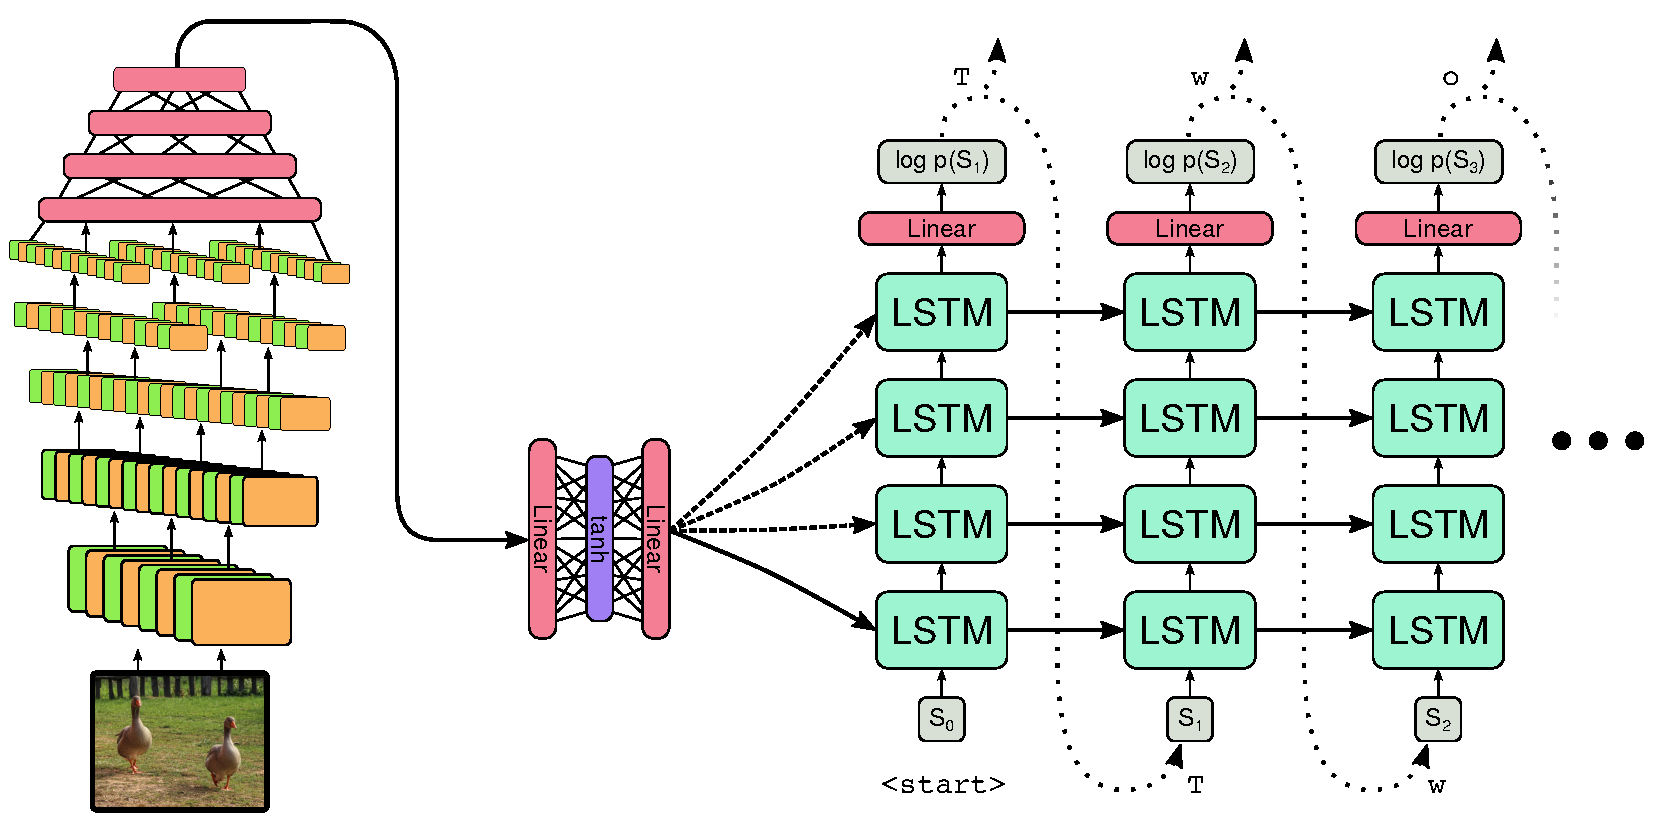
\includegraphics[width=0.75\textwidth]{./fig/proposed-model.pdf}
	\caption{Architecture of the proposed model.
		\label{fig:proposedModel}}
\end{figure}

First question, this architecture is supposed to answer, is, whether model without the support of embeddings can compete with other contemporary solutions. Second is, how much will the model improve, if LSTM units are set with a large bias, as described in \cite{DBLP:conf/icml/JozefowiczZS15} and in part \ref{subsec:gru}.

Model will work with one-hot character level encoding, with two extra special characters \texttt{<start>} and \texttt{<stop>}, which respectively mark beginning and the end of sequence. Size of the first LSTM layer will be between $ 100-1000 $ items, number similar to the image embedding models mentioned in \cite{DBLP:journals/corr/VinyalsTBE14, DBLP:journals/corr/FangGISDDGHMPZZ14}.

Training will be performed on MS COCO and Flickr datasets, mentioned in part \ref{sec:datasets}. I would also like to explore Adam\cite{DBLP:journals/corr/KingmaB14} and several other optimization algorithms.

%\chapter{Implementation}
%\todo[inline, color=cyan!60]{Bude az v diplomce, ne semestralnim projektu}
%
%	\section{Torch framework}
%\todo[inline]{Popis Torche, ruznych druhu modulu ktere ma, ktere jsem pouzil ja.}
%
%	\section{Parallelization}
%\todo[inline]{Nejaky popis toho ze to lze trenovat na gpu, jak se to dela v Torchi..}	
%
%\chapter{Results and model evaluation}
%\todo[inline, color=cyan!60]{Bude az v diplomce, ne semestralnim projektu}
%\todo[inline]{Performance, analysis,... spravne pojmenovat}
%\todo[inline]{Kde se trenovalo? Na jakych strojich? Jak to bylo rychle? Jak to bylo na cpu pomale?}
%
%	\section{Speed}
%\todo[inline]{Jak bylo trenovani rychle, }

\chapter{Conclusion}\label{chp:conclusion}

Image captioning is problem more difficult than simple classification of images. Nowadays, deep neural networks are dominating the field almost exclusively. In this work I explained several features of neural networks, which are necessary for creation of image captioning models, and created an overview of state-of-the-art approaches to this problem. Deep learning is research area with a great need of data, therefore I also listed several biggest and most commonly used datasets and evaluation methods.

Character level prediction models were created as a building block for creating my own image captioning model, based on the information compiled. I proposed an architecture of the model based on several other approaches, with interest in character level language models instead of word embedding. I explore whether this simple architecture can compete with contemporary solutions focused on word level language models.

In several following months I am planning to work on the details of the convolutional network architecture, implementation and training of the proposed model. Project should be finished by May 2016.


%=========================================================================
